\section{The implementation}
	\paragraph{}
	There are many technologies that allow building web applications, and they are divided into two main parts, the front-end part such as HTML, CSS, JS ..., and the back-end part such as PHP, NodeJS ..., in addition to databases, but we will depend in our project on the following:
	\subsection{Implementation Technologies}
		\subsubsection{For front-end}
			\paragraph{HTML}
			HTML (Hyper-Text Markup Language) is the standard mark-up language for documents designed to be displayed in a web browser. It can be assisted by technologies such as Cascading Style Sheets (CSS) and scripting languages such as JavaScript.\cite{HTML}
			\paragraph{CSS}
			Cascading Style Sheets (CSS) is a simple mechanism for adding style (e.g., fonts, colors, spacing) to Web documents.\cite{CSS}
			\paragraph{Bootstrap}
			The world’s most popular front-end open source toolkit, featuring Sass variables and mixins, responsive grid system, extensive prebuilt components, and powerful JavaScript plugins.\cite{Bootstrap}
		\subsubsection{For back-end}
			\paragraph{Django Web Framework}
			Django is a high-level Python Web framework that encourages rapid development and clean, pragmatic design. Built by experienced developers, it takes care of much of the hassle of Web development, so you can focus on writing your app without needing to reinvent the wheel. It’s free and open source.\cite{Django}
			\paragraph{why django ?}
			\begin{itemize}
				\item It's a Python Language.
				\item Easy to learn.
				\item Fast and secured.
				\item Built-in administration interface.
				\item Framework able to customization.
				\item large community.
				\item MVC design pattern.
				\item Built-in ORM for databases.
				\item and much more ...
			\end{itemize}
		
			\paragraph{PostgreSQL}
			PostgreSQL is a powerful, open source object-relational database system with over 30 years of active development that has earned it a strong reputation for reliability, feature robustness, and performance.\cite{PostgreSQL}
	
	\subsection{Interfaces of the site}
	
	\subsubsection{Index Page}
		\paragraph{}
		In Figure \ref{fig:home-before-login} we see home page of the site for the user who haven't logged in.
		
			\begin{figure}[b]
				\centering
				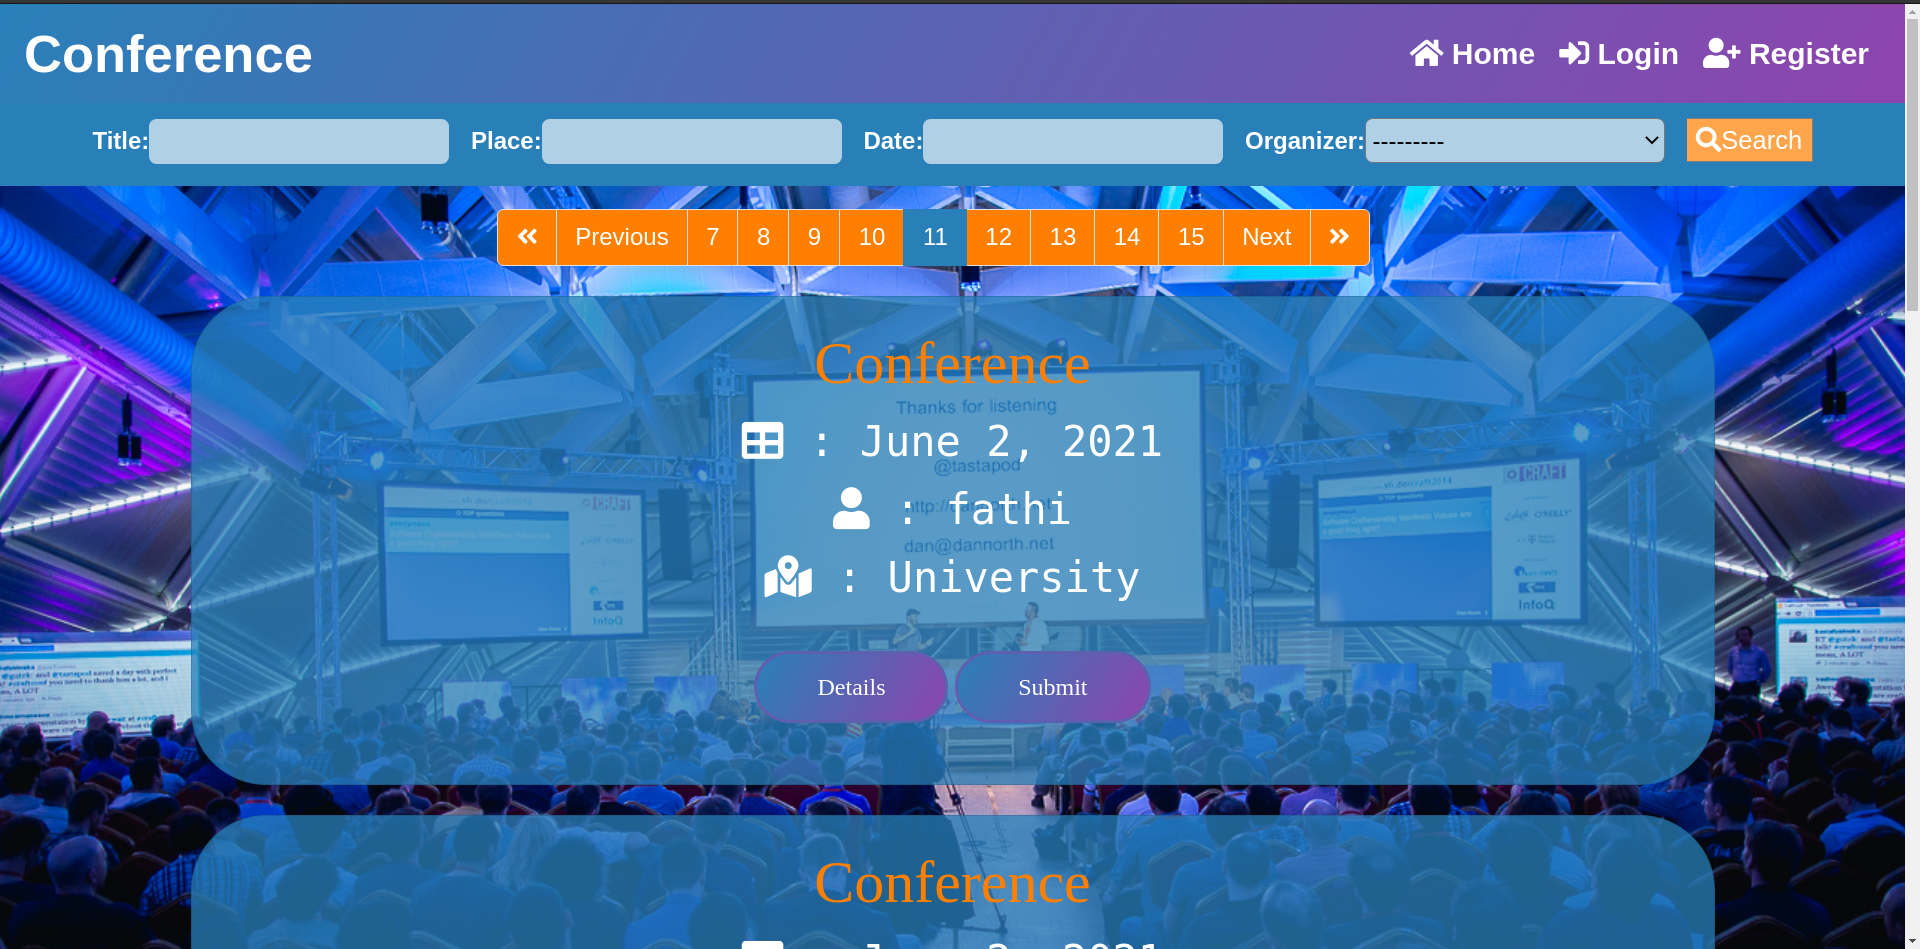
\includegraphics[width=\textwidth]{interfaces/before_login.png}
				\caption{Home page for guests}
				\label{fig:home-before-login}
			\end{figure}

		\paragraph{}
		In Figure \ref{fig:home-after-login} we see home page of the site for the user who have logged in.
		
			\begin{figure}[b]
				\centering
				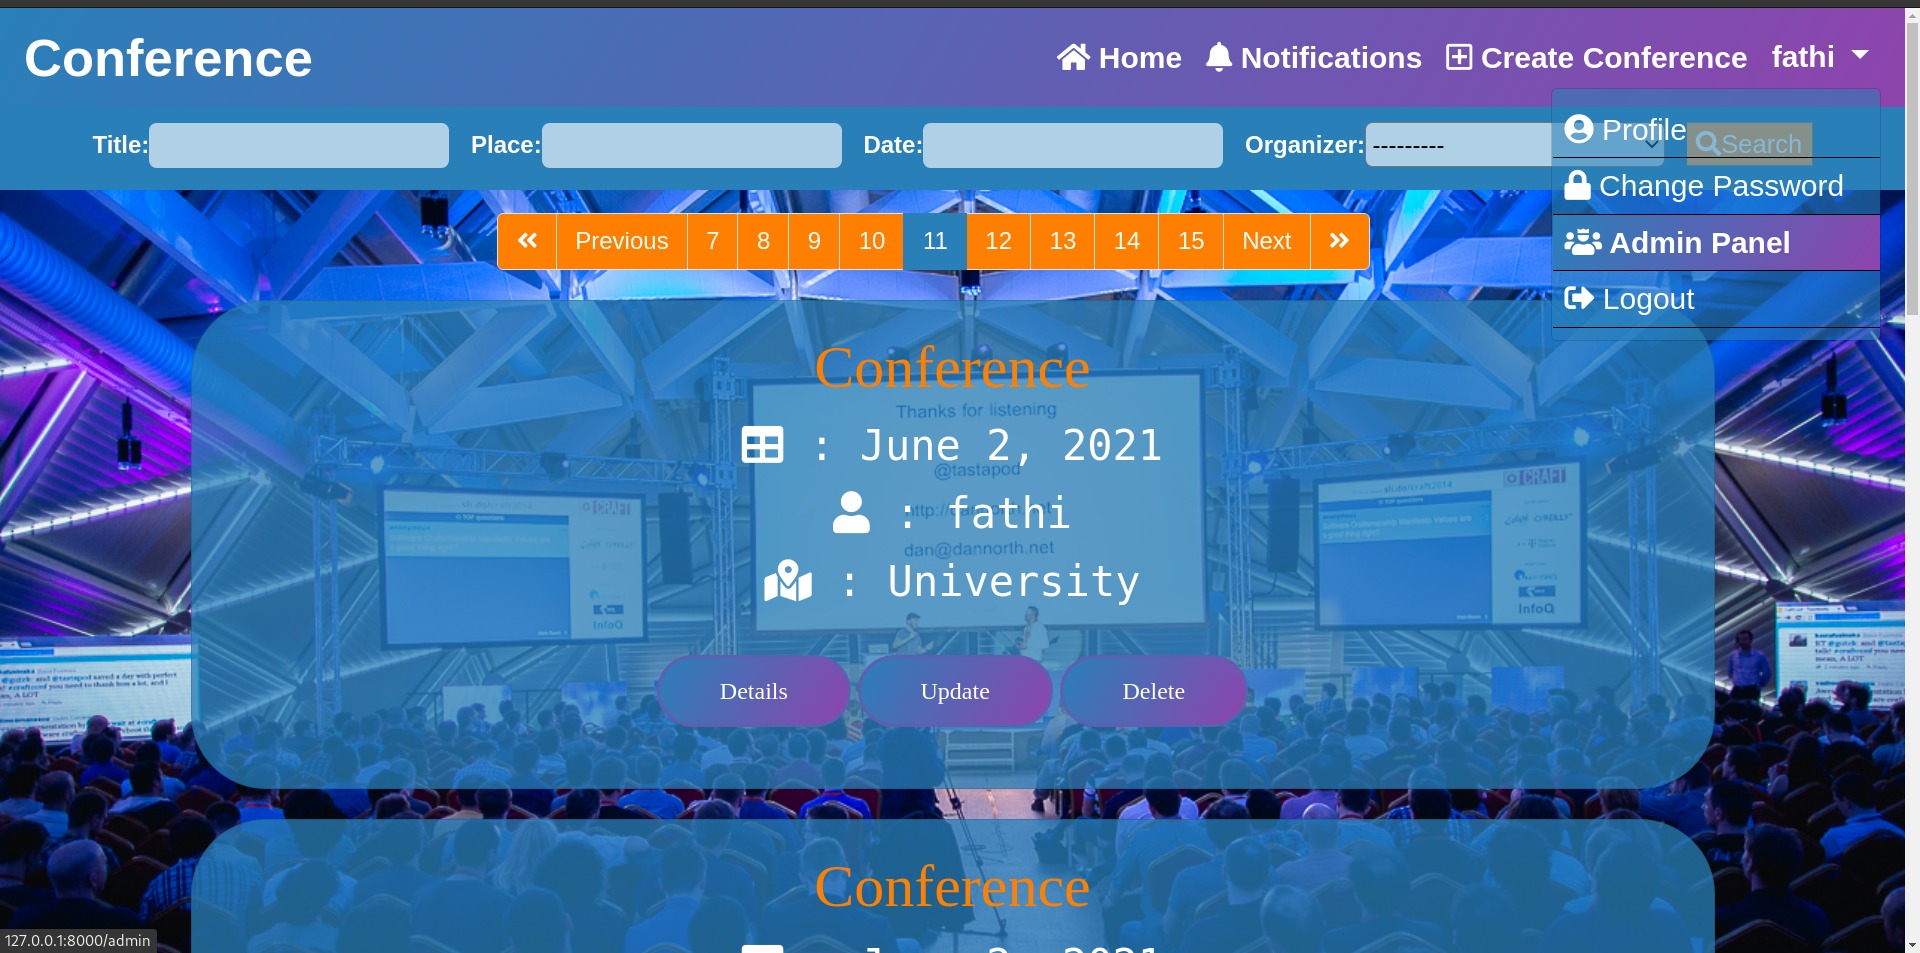
\includegraphics[width=\textwidth]{interfaces/after_login.png}
				\caption{Home page for registered users}
				\label{fig:home-after-login}
			\end{figure}

	\subsubsection{Conference Details page}
		\paragraph{}
		In Figure \ref{fig:details-organizer} we see a conference details page when the logged in user is the organizer.
		
			\begin{figure}[b]
				\centering
				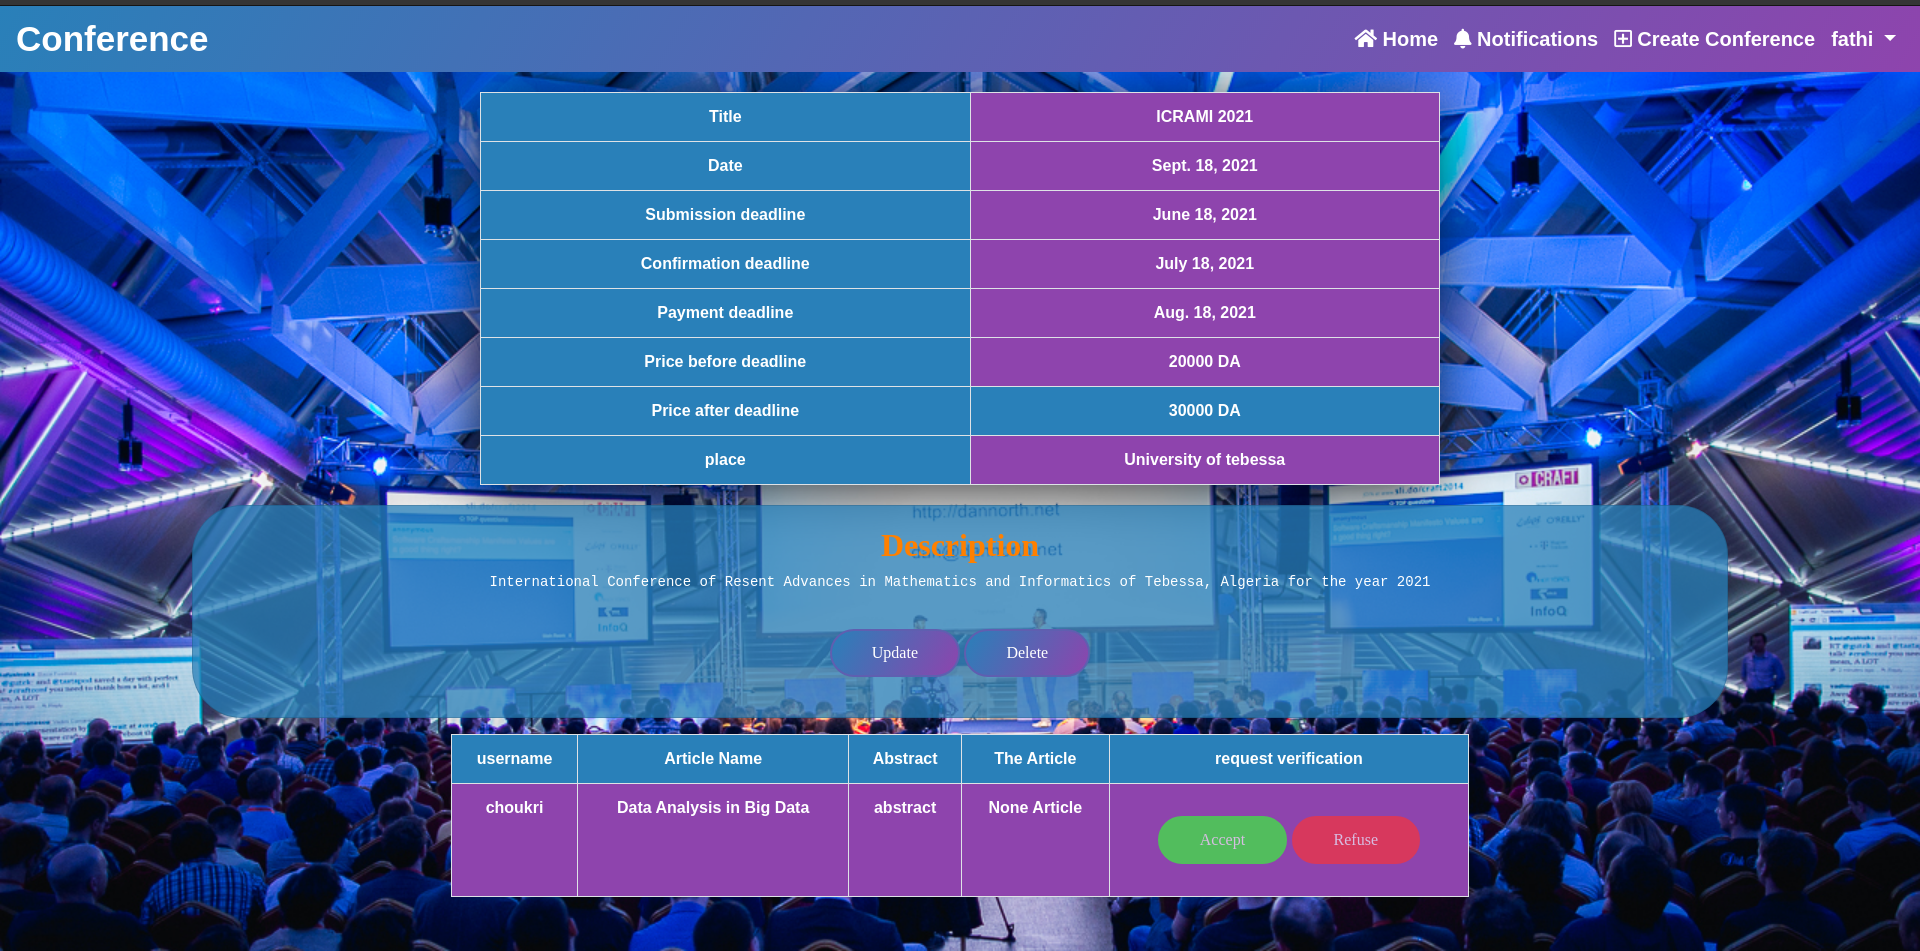
\includegraphics[width=\textwidth]{interfaces/details_organizer.png}
				\caption{Conference Details page for its organizer}
				\label{fig:details-organizer}
			\end{figure}

		\paragraph{}
		In Figure \ref{fig:details-non-organizer} we see a conference details page when the logged in user isn't the organizer.
		
			\begin{figure}[b]
				\centering
				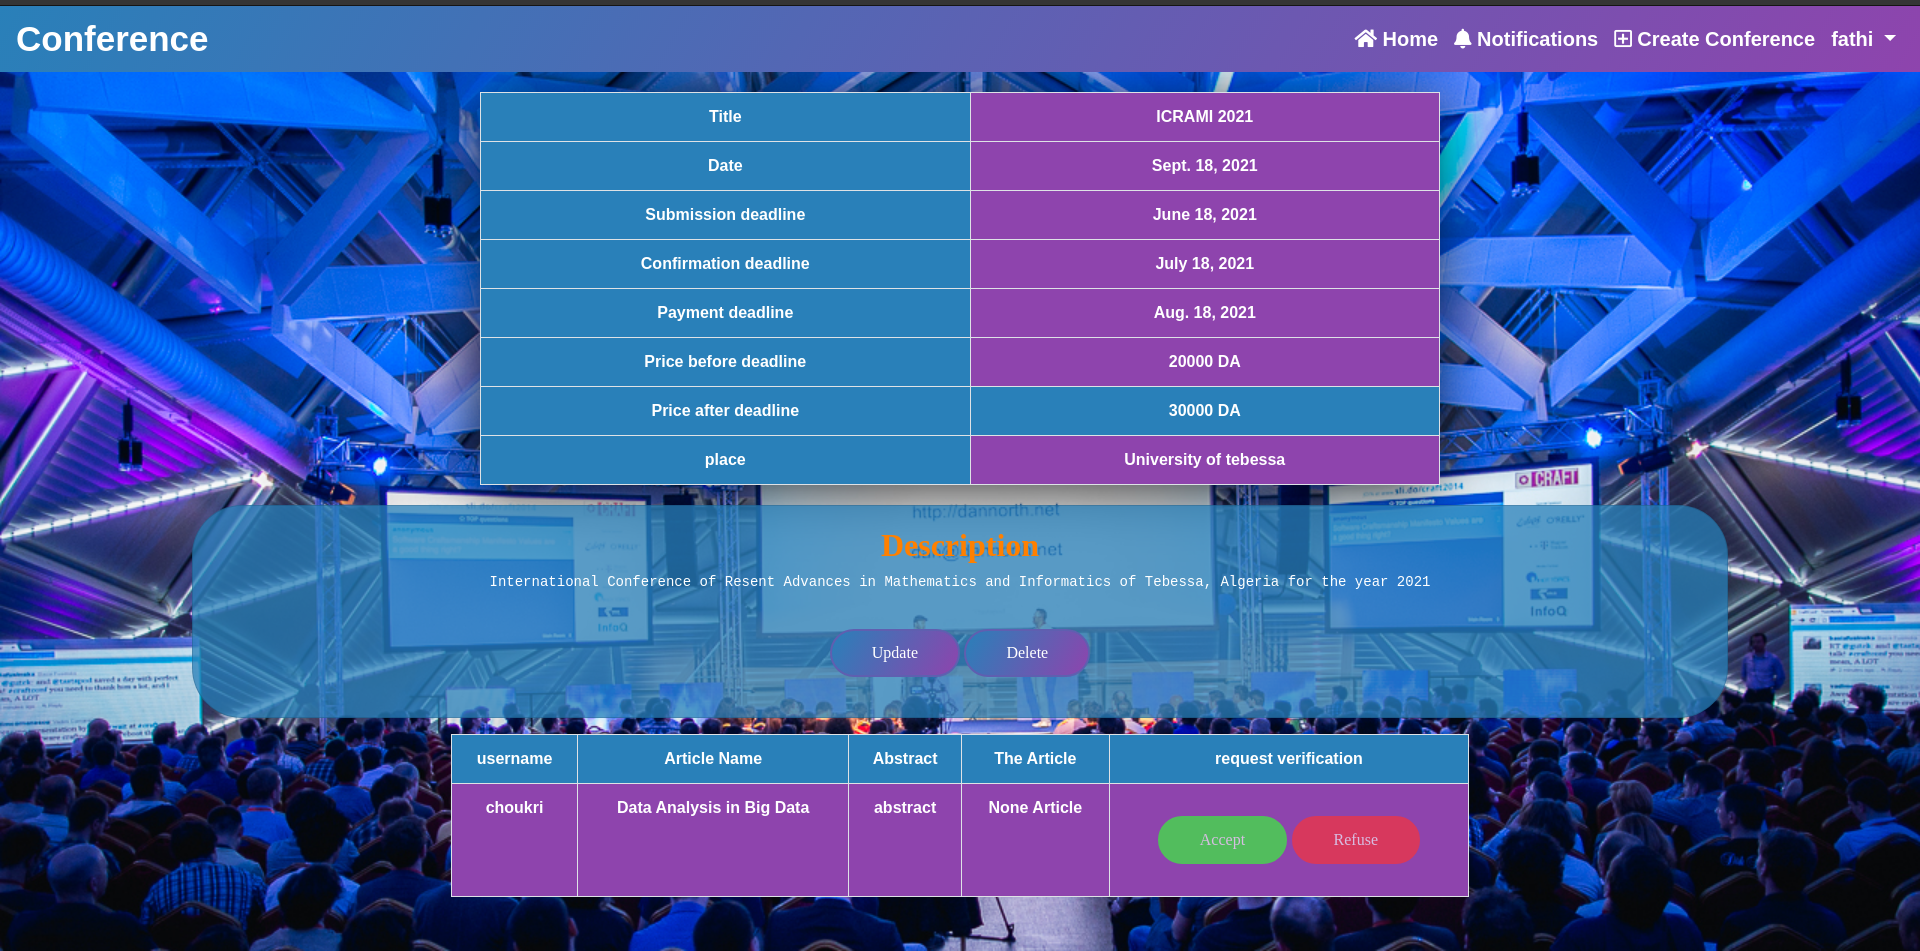
\includegraphics[width=\textwidth]{interfaces/details_organizer.png}
				\caption{Conference Details page for its organizer}
				\label{fig:details-non-organizer}
			\end{figure}

	\subsubsection{Notifications page}
		\paragraph{}
		In Figure \ref{fig:notifications} we see notifications page.
		
			\begin{figure}
				\centering
				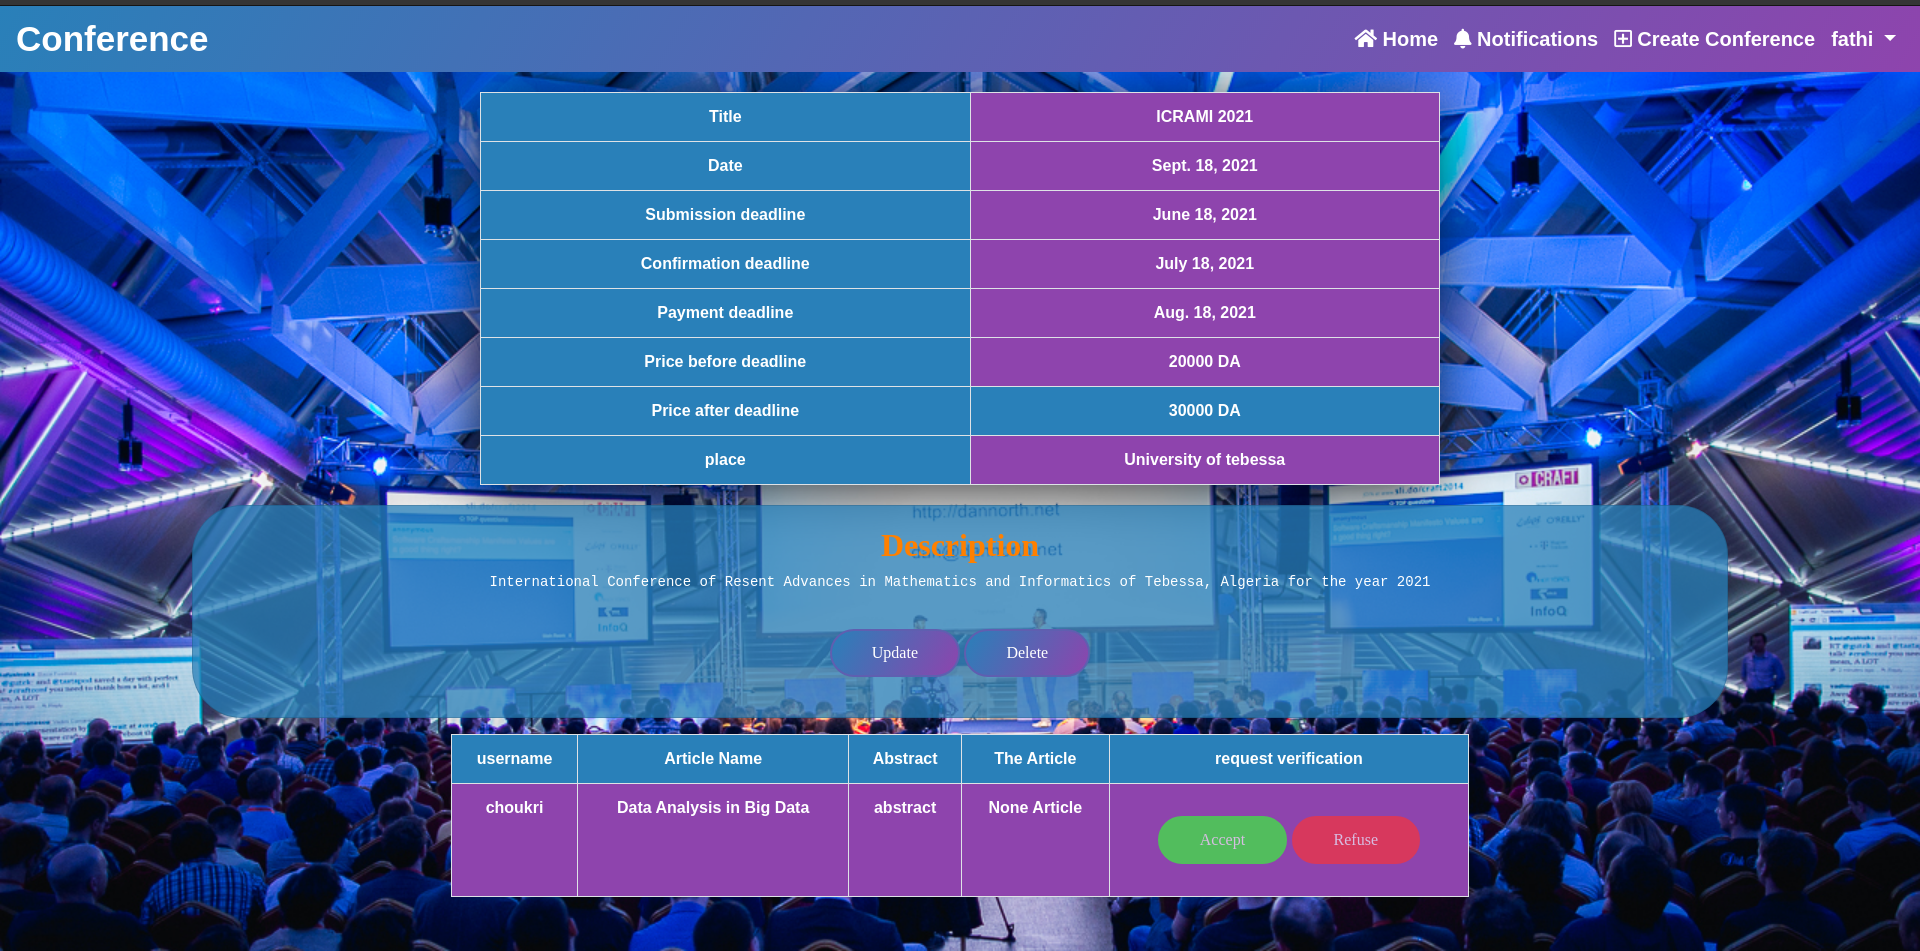
\includegraphics[width=\textwidth]{interfaces/details_organizer.png}
				\caption{Noifications page}
				\label{fig:notifications}
			\end{figure}

	\subsubsection{Conference Creation page}
		\paragraph{}
		In Figure \ref{fig:new-conf} we see the page of conference creation.
		
			\begin{figure}
				\centering
				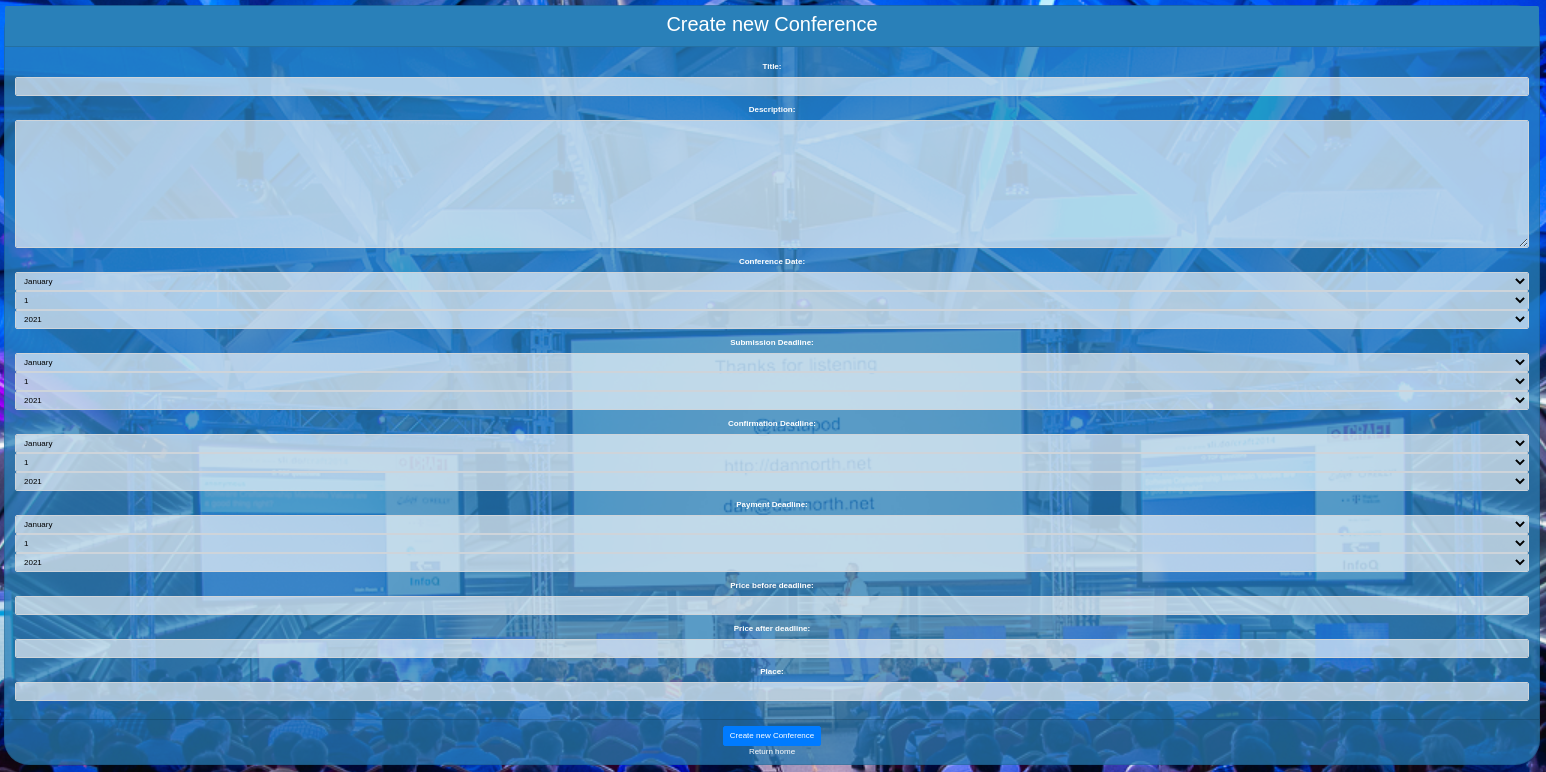
\includegraphics[width=\textwidth]{interfaces/new_conference.png}
				\caption{Conference Creation page}
				\label{fig:new-conf}
			\end{figure}
	
	\subsubsection{Conference Creation page}
		\paragraph{}
		In Figure \ref{fig:new-sub} we see the page of submission creation.
		
			\begin{figure}
				\centering
				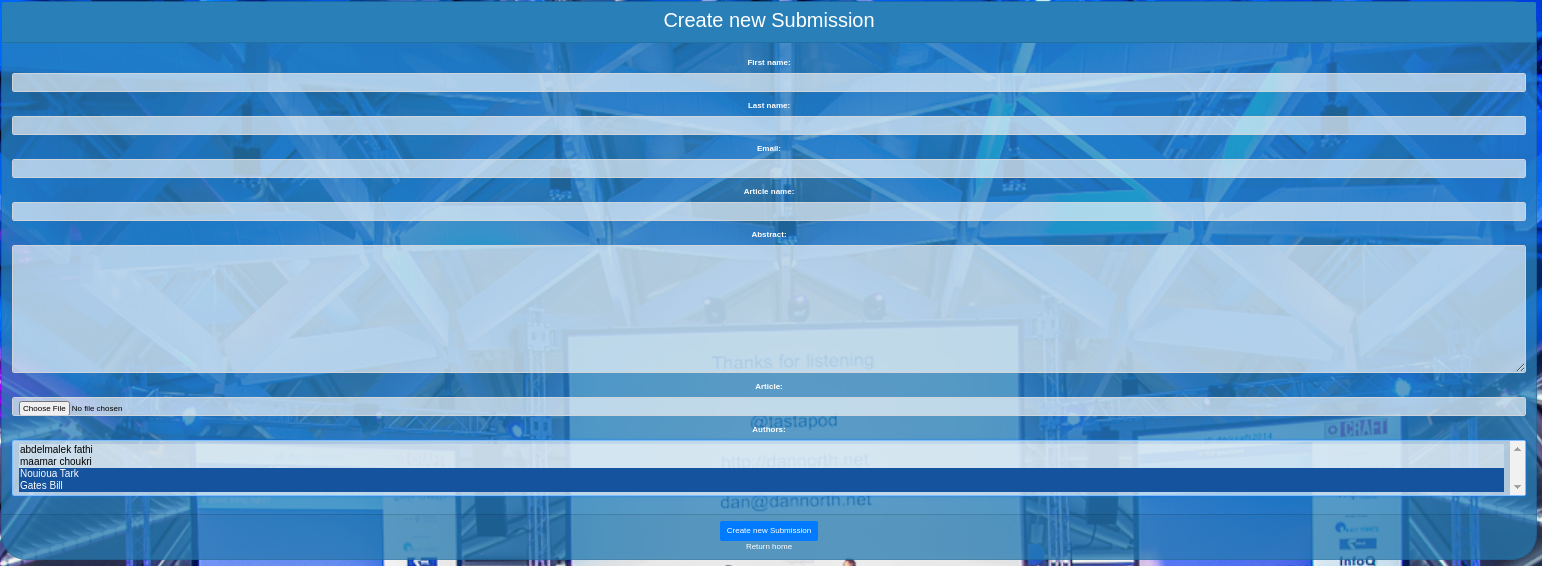
\includegraphics[width=\textwidth]{interfaces/new_submission.png}
				\caption{Submission Creation page}
				\label{fig:new-sub}
			\end{figure}